\documentclass{article}

% --- Packages ---
\usepackage[preprint]{neurips_2024}
\usepackage[utf8]{inputenc}
\usepackage[T1]{fontenc}
\usepackage{hyperref}
\usepackage{url}
\usepackage{booktabs}
\usepackage{amsmath}
\usepackage{graphicx}
\usepackage{subcaption}
\usepackage{multirow}
\usepackage{xcolor}
\usepackage{microtype}
\usepackage{natbib}

\definecolor{swcolor}{HTML}{888780}
\definecolor{sqlcolor}{HTML}{378ADD}
\definecolor{veccolor}{HTML}{D85A30}

% ---------------------------------------------------------------------------
\title{Memory Retrieval Strategy Matters:\\
A Comparative Study of Episodic Memory Backends\\
for Reflexion-Style LLM Agents}

\author{
  Shilo Jeyarajasingam \\
  University of Waterloo $\cdot$ Independent Researcher \\
  \texttt{stjeyara@uwaterloo.ca}
}

\begin{document}
\maketitle

% ---------------------------------------------------------------------------
\begin{abstract}
Reflexion \citep{shinn2023reflexion} improves large language model (LLM)
performance through iterative self-reflection, storing verbal lessons in an
episodic memory buffer. We show that a retrieval ordering decision within a
backend class accounts for a larger performance gap than the choice of backend
itself: surfacing failure episodes first rather than successes first yields a
12 percentage point improvement in success@5 on multi-step reasoning, a
non-obvious result with direct practical implications for any practitioner
building memory-augmented agents. A Vector DB with semantic similarity
retrieval achieves the highest first-attempt success rate (70.0\% vs.\
58.0\% for other backends) and lowest token cost, consistent with the
hypothesis that semantically similar past tasks share applicable lessons.
Once the ordering decision is corrected, SQL and Vector DB converge to
equivalent success@5 (84\%), both outperforming the sliding-window baseline
on first-attempt accuracy. The tool-use domain exhibits a ceiling effect
(100\% success@5 across all backends), highlighting the need for harder
benchmarks to differentiate memory backend performance. A GPT-4o-mini
replication on the reasoning domain confirms these patterns are
model-agnostic: success@5 gaps narrow to within 4pp across all three
backends despite substantially lower first-attempt accuracy. We release
all code, result data, and experimental configurations at
\url{https://github.com/shilojeyaraj/reflexion-memory-study}.
\end{abstract}

% ---------------------------------------------------------------------------
\section{Introduction}
\label{sec:intro}

Large language models can improve their own performance on sequential tasks
through self-generated verbal feedback, a process formalised by Reflexion
\citep{shinn2023reflexion}. After each failed attempt, the agent reflects on
its error, stores a verbal lesson in memory, and retrieves that lesson on
subsequent attempts. The quality of this feedback loop depends on two
components: the \emph{reflector} that generates lessons, and the
\emph{memory backend} that stores and retrieves them.

The original Reflexion paper evaluates the reflector extensively but treats
the memory backend as a fixed implementation detail: a sliding window of the
$k$ most recent episodes. This design is simple and requires no external
infrastructure, but it has a fundamental limitation. Retrieval is
\emph{recency-ordered only}. If a relevant past lesson occurred more than $k$
episodes ago, it is silently discarded. As the agent accumulates experience
across many tasks, the gap between available lessons and actually retrieved
lessons grows.

We hypothesise that more principled retrieval strategies can improve sample
efficiency and task success. Specifically:

\begin{itemize}
  \item \textbf{SQL (structured retrieval):} Filtering by domain and error
    type surfaces the subset of stored episodes most likely to be relevant
    to the current failure mode, maintaining precision as the database grows.
  \item \textbf{Vector DB (semantic retrieval):} Embedding-based similarity
    search identifies lessons from semantically related tasks regardless of
    recency or error category, enabling cross-task generalisation.
\end{itemize}

We make the following contributions:
\begin{enumerate}
  \item The discovery that retrieval ordering within a backend class accounts
    for a larger performance gap (12 percentage points) than the choice of
    backend itself. This is a non-obvious finding with immediate practical
    value for any practitioner building memory-augmented agents.
  \item Empirical evidence that Vector DB achieves higher first-attempt
    success and lower token cost on reasoning tasks, consistent with the
    semantic retrieval hypothesis.
  \item A signal-to-noise framework for reasoning about backend choice as a
    function of task structure and database size.
  \item A reproducible experimental framework comparing three memory backends
    across two task domains using only open-source tools (SQLite, ChromaDB,
    HotpotQA, BFCL).
\end{enumerate}

% ---------------------------------------------------------------------------
\section{Related Work}
\label{sec:related}

\paragraph{Reflexion.}
\citet{shinn2023reflexion} introduce Reflexion, in which an LLM agent
verbalises lessons learned from task failures and stores them in an episodic
buffer. Retrieved lessons augment the agent's context on subsequent attempts.
The original work uses a fixed-size sliding window and evaluates on HotpotQA,
AlfWorld, and HumanEval. Our work extends this by studying the memory
component directly, treating retrieval strategy as the independent variable.

\paragraph{Memory-augmented language agents.}
MemGPT \citep{packer2023memgpt} proposes a hierarchical memory architecture
for LLM agents, distinguishing in-context, external, and archival memory
tiers. \citet{zhong2024memorybank} introduce MemoryBank, a long-term memory
system using vector retrieval for personalised LLM assistants.
\citet{park2023generative} demonstrate episodic memory retrieval in generative
agent simulations. Our work differs in focus: we study how retrieval strategy
interacts with the specific \emph{self-improvement} mechanism of Reflexion,
where retrieved content is verbal lessons rather than factual knowledge.

\paragraph{Retrieval-augmented generation.}
RAG systems \citep{lewis2020retrieval} retrieve external documents to augment
LLM responses. Dense passage retrieval \citep{karpukhin2020dense} and
contrastive learning-based embeddings \citep{reimers2019sentencebert} underpin
modern semantic retrieval. Our vector backend uses sentence-transformers
\citep{reimers2019sentencebert} for embedding reflection text, applying RAG
principles to the agent self-improvement setting.

\paragraph{Tool-use and function calling benchmarks.}
The Berkeley Function-Calling Leaderboard (BFCL; \citealt{yan2024bfcl})
provides standardised evaluation of LLM function-calling accuracy using AST
matching. We evaluate on BFCL's \emph{multiple\_function} split, which
requires the agent to select the correct function from a candidate set with
similar signatures. Despite this harder disambiguation requirement, a 100\%
success@5 ceiling persists across all backends, indicating that GPT-4o
solves these tasks reliably without needing memory-assisted iteration.
Sequential multi-tool benchmarks such as ToolBench \citep{qin2023toolllm}
are likely needed to create the graded signal required for backend
differentiation.

\paragraph{Multi-step reasoning.}
HotpotQA \citep{yang2018hotpotqa} requires multi-hop reasoning over Wikipedia
passages. We use the distractor setting, which provides 10 candidate passages
per question, matching the format used by Reflexion.

% ---------------------------------------------------------------------------
\section{Methods}
\label{sec:methods}

\subsection{Memory Backends}

We implement three backends, each conforming to a common
\texttt{MemoryBackend} interface with \texttt{store()}, \texttt{retrieve()},
and \texttt{reset()} methods.

\paragraph{Sliding Window (baseline).}
Episodes are stored in a Python list. \texttt{retrieve(query, k)} ignores
the query entirely and returns the $k$ most recent episodes. This mirrors
the original Reflexion implementation. No persistence is used; all state
is held in-process.

\paragraph{SQL (SQLite).}
Episodes are stored in a local SQLite database (zero external dependencies,
sub-millisecond retrieval). \texttt{retrieve(query, k)} filters by domain
and returns $k$ episodes ordered by \texttt{success ASC, timestamp DESC}:
failures first, most recent first within each group. On attempt $t \geq 2$,
the actor calls \texttt{retrieve\_by\_error\_type(prev\_error\_type, k)} to
surface episodes sharing the exact failure mode of the previous attempt,
falling back to general domain retrieval if fewer than $k$ error-type
matches exist.

\paragraph{Vector DB (ChromaDB).}
Episodes are embedded using \texttt{all-MiniLM-L6-v2}
\citep{reimers2019sentencebert} from the sentence-transformers library.
The embedded string is
\texttt{"{domain}: {action\_summary} -> {reflection}"}. \texttt{retrieve(query,
k)} embeds the current task description and returns the $k$ nearest
neighbours by cosine similarity, subject to a minimum similarity threshold
of 0.55. A persistent ChromaDB collection is used across tasks within a
single experimental run.

\subsection{Experimental Setup}

\paragraph{Models.}
We evaluate two models to assess whether findings generalise across
capability levels. The primary model is GPT-4o (\texttt{gpt-4o}), used for
all conditions. The secondary model is GPT-4o-mini (\texttt{gpt-4o-mini}),
run on the reasoning domain only to test whether the SQL retrieval ordering
effect is model-agnostic. We set temperature to the API default (1.0) for
both models.

\paragraph{Trial loop.}
Each task runs for up to 5 attempts. On each attempt: (1) the actor
retrieves $k{=}3$ past reflections and generates a response; (2) the
environment evaluates the response and returns (reward, success, feedback,
error\_type); (3) the reflector generates a verbal lesson; (4) the episode
is stored in memory. The loop terminates on success or after 5 attempts.

\paragraph{Domains and benchmarks.}

\emph{Reasoning (HotpotQA):} We sample 50 questions from the distractor
validation split using a fixed seed. Reward is 1.0 for exact match, 0.5
for substring match, and 0.0 otherwise. Error types: \texttt{exact\_match},
\texttt{partial\_match}, \texttt{wrong\_answer}.

\emph{Tool-use (BFCL multiple\_function):} We use all 20 available tasks
from the BFCL \texttt{multiple\_function} split \citep{yan2024bfcl}, which
requires selecting the correct function from among candidates with similar
names and signatures. The agent outputs Python function call syntax;
correctness is evaluated by AST matching against the reference call.
Reward is binary (1.0/0.0). Error types: \texttt{success},
\texttt{wrong\_function}, \texttt{wrong\_args}, \texttt{type\_error},
\texttt{ambiguous\_selection}.

\paragraph{Note on code domain.}
The HumanEval benchmark \citep{chen2021humaneval} was excluded because its
execution harness relies on \texttt{signal.SIGALRM}, which is unavailable
on Windows. Results therefore cover two of the original three Reflexion
domains.

\paragraph{Infrastructure.}
SQLite is used in preference to hosted PostgreSQL to eliminate network
latency as a confound in token and cost metrics, and to ensure full
reproducibility from \texttt{git clone} with no credentials required. All
experiments ran on a single machine; no distributed infrastructure was used.

\subsection{Metrics}

\begin{itemize}
  \item \textbf{success@k}: fraction of tasks solved within $k$ attempts.
  \item \textbf{sample efficiency}: number of episodes until 70\% of tasks
    are solved (lower is better; $\infty$ if never reached).
  \item \textbf{mean tokens per task}: average total token consumption
    across all attempts for a task.
  \item \textbf{cost per solved task}: estimated USD cost (\$0.005 per 1k
    tokens, blended GPT-4o rate) divided by number of solved tasks.
\end{itemize}

Statistical significance is assessed using the Wilcoxon signed-rank test
on per-task binary success@5 scores, with $p < 0.05$ as the significance
threshold.

% ---------------------------------------------------------------------------
\section{Results}
\label{sec:results}

\begin{table}[t]
\centering
\caption{
  Main results across memory backends and task domains.
  SW = Sliding Window; SQL-v1 = SQL with success-first retrieval (original,
  with ordering error); SQL-v2 = SQL with failure-first retrieval
  (corrected); Vec = Vector DB. Best per domain in \textbf{bold}.
  $n{=}50$ for reasoning; $n{=}20$ for tool-use (all available
  \texttt{multiple\_function} tasks).
}
\label{tab:main}
\small
\begin{tabular}{llccccc}
\toprule
Domain & Backend & success@1 & success@3 & success@5
  & Mean tokens & Cost/solved (\$) \\
\midrule
\multirow{4}{*}{Reasoning}
  & SW       & 0.580 & \textbf{0.840} & \textbf{0.860}
             & 3{,}967 & 0.0152 \\
  & SQL-v1   & 0.580 & 0.700          & 0.720
             & 4{,}649 & 0.0134 \\
  & SQL-v2   & 0.580 & 0.780          & 0.840
             & 4{,}076 & 0.0151 \\
  & Vec      & \textbf{0.700} & 0.820 & 0.840
             & \textbf{3{,}621} & \textbf{0.0125} \\
\midrule
\multirow{3}{*}{Tool-use}
  & SW       & \textbf{1.000} & \textbf{1.000} & \textbf{1.000}
             & \textbf{966} & \textbf{0.0048} \\
  & SQL-v2   & 0.950          & \textbf{1.000} & \textbf{1.000}
             & 1{,}037 & 0.0052 \\
  & Vec      & \textbf{1.000} & \textbf{1.000} & \textbf{1.000}
             & 1{,}016 & 0.0051 \\
\bottomrule
\end{tabular}
\end{table}

\subsection{Reasoning Domain (HotpotQA)}

Results are shown in Table~\ref{tab:main}. Three findings stand out.

\paragraph{Vector DB leads on first-attempt success.}
Vec achieves 70.0\% success@1 versus 58.0\% for SW and both SQL variants,
a 12 percentage point advantage. This is consistent with the semantic
retrieval hypothesis: HotpotQA questions cluster by topic and reasoning
pattern, so semantically similar past tasks share applicable lessons
regardless of recency. The actor, presented with relevant prior reflections
on attempt 1, resolves more tasks without needing any retry. Vec also
achieves the lowest mean token count (3{,}621) and lowest cost per solved
task (\$0.0125), suggesting the retrieved reflections are high-signal
enough to reduce response length and retry overhead.

\paragraph{Sliding Window leads on success@5.}
SW achieves 86.0\% success@5, narrowly outperforming SQL-v2 and Vec (both
84.0\%), though the difference is not statistically significant
($p = 0.317$, Wilcoxon). This is consistent with the dataset structure:
with a fixed shuffle seed, similar HotpotQA question types cluster together
in task order, making recent episodes incidentally relevant. This is a
dataset artefact rather than a principled advantage of recency-based
retrieval.

\paragraph{SQL-v1 significantly underperforms; SQL-v2 recovers.}
SQL-v1 achieves only 72.0\% success@5, significantly below SW ($p = 0.020$)
and Vec ($p = 0.034$). Post-hoc audit revealed the cause: SQL-v1's
\texttt{ORDER BY success DESC} retrieval surfaced 351 of 353 retrieved
episodes with \texttt{error\_type = exact\_match} (i.e.\ past successes).
The agent was shown reminders of what had worked before rather than lessons
from failures, effectively inverting the Reflexion mechanism. Correcting
the ordering to \texttt{success ASC, timestamp DESC} (failure-first)
recovers 12 percentage points, bringing SQL-v2 to 84.0\%, which is
statistically indistinguishable from Vec ($p = 1.000$). The SQL-v1
vs.\ SQL-v2 comparison is a controlled ablation: all other variables
(schema, filtering logic, embedding, model) are held constant. Only
retrieval ordering changes.

\subsection{SQL Retrieval Ordering Ablation}
\label{sec:ordering}

Figure~\ref{fig:ordering} shows the success curves for all four reasoning
conditions across trial numbers 1--5. SQL-v1 diverges from the other
backends at trial 2 and continues to lag throughout: tasks that reached
attempt 2 were being shown successful past episodes rather than
failure-specific lessons, preventing the agent from correctly diagnosing
its error type. By trial 5, SQL-v1 has 15 tasks still failing (compared
to 7 for SW and 8 for Vec/SQL-v2), all cycling through
\texttt{partial\_match} and \texttt{wrong\_answer} errors without
improvement.

This result has a practical implication: for any Reflexion-style system
using structured memory, retrieval must prioritise failure episodes.
Success episodes are valuable as \emph{few-shot exemplars} but
counterproductive for \emph{error diagnosis}, which is what Reflexion's
reflector requires.

\begin{figure}[h]
\centering
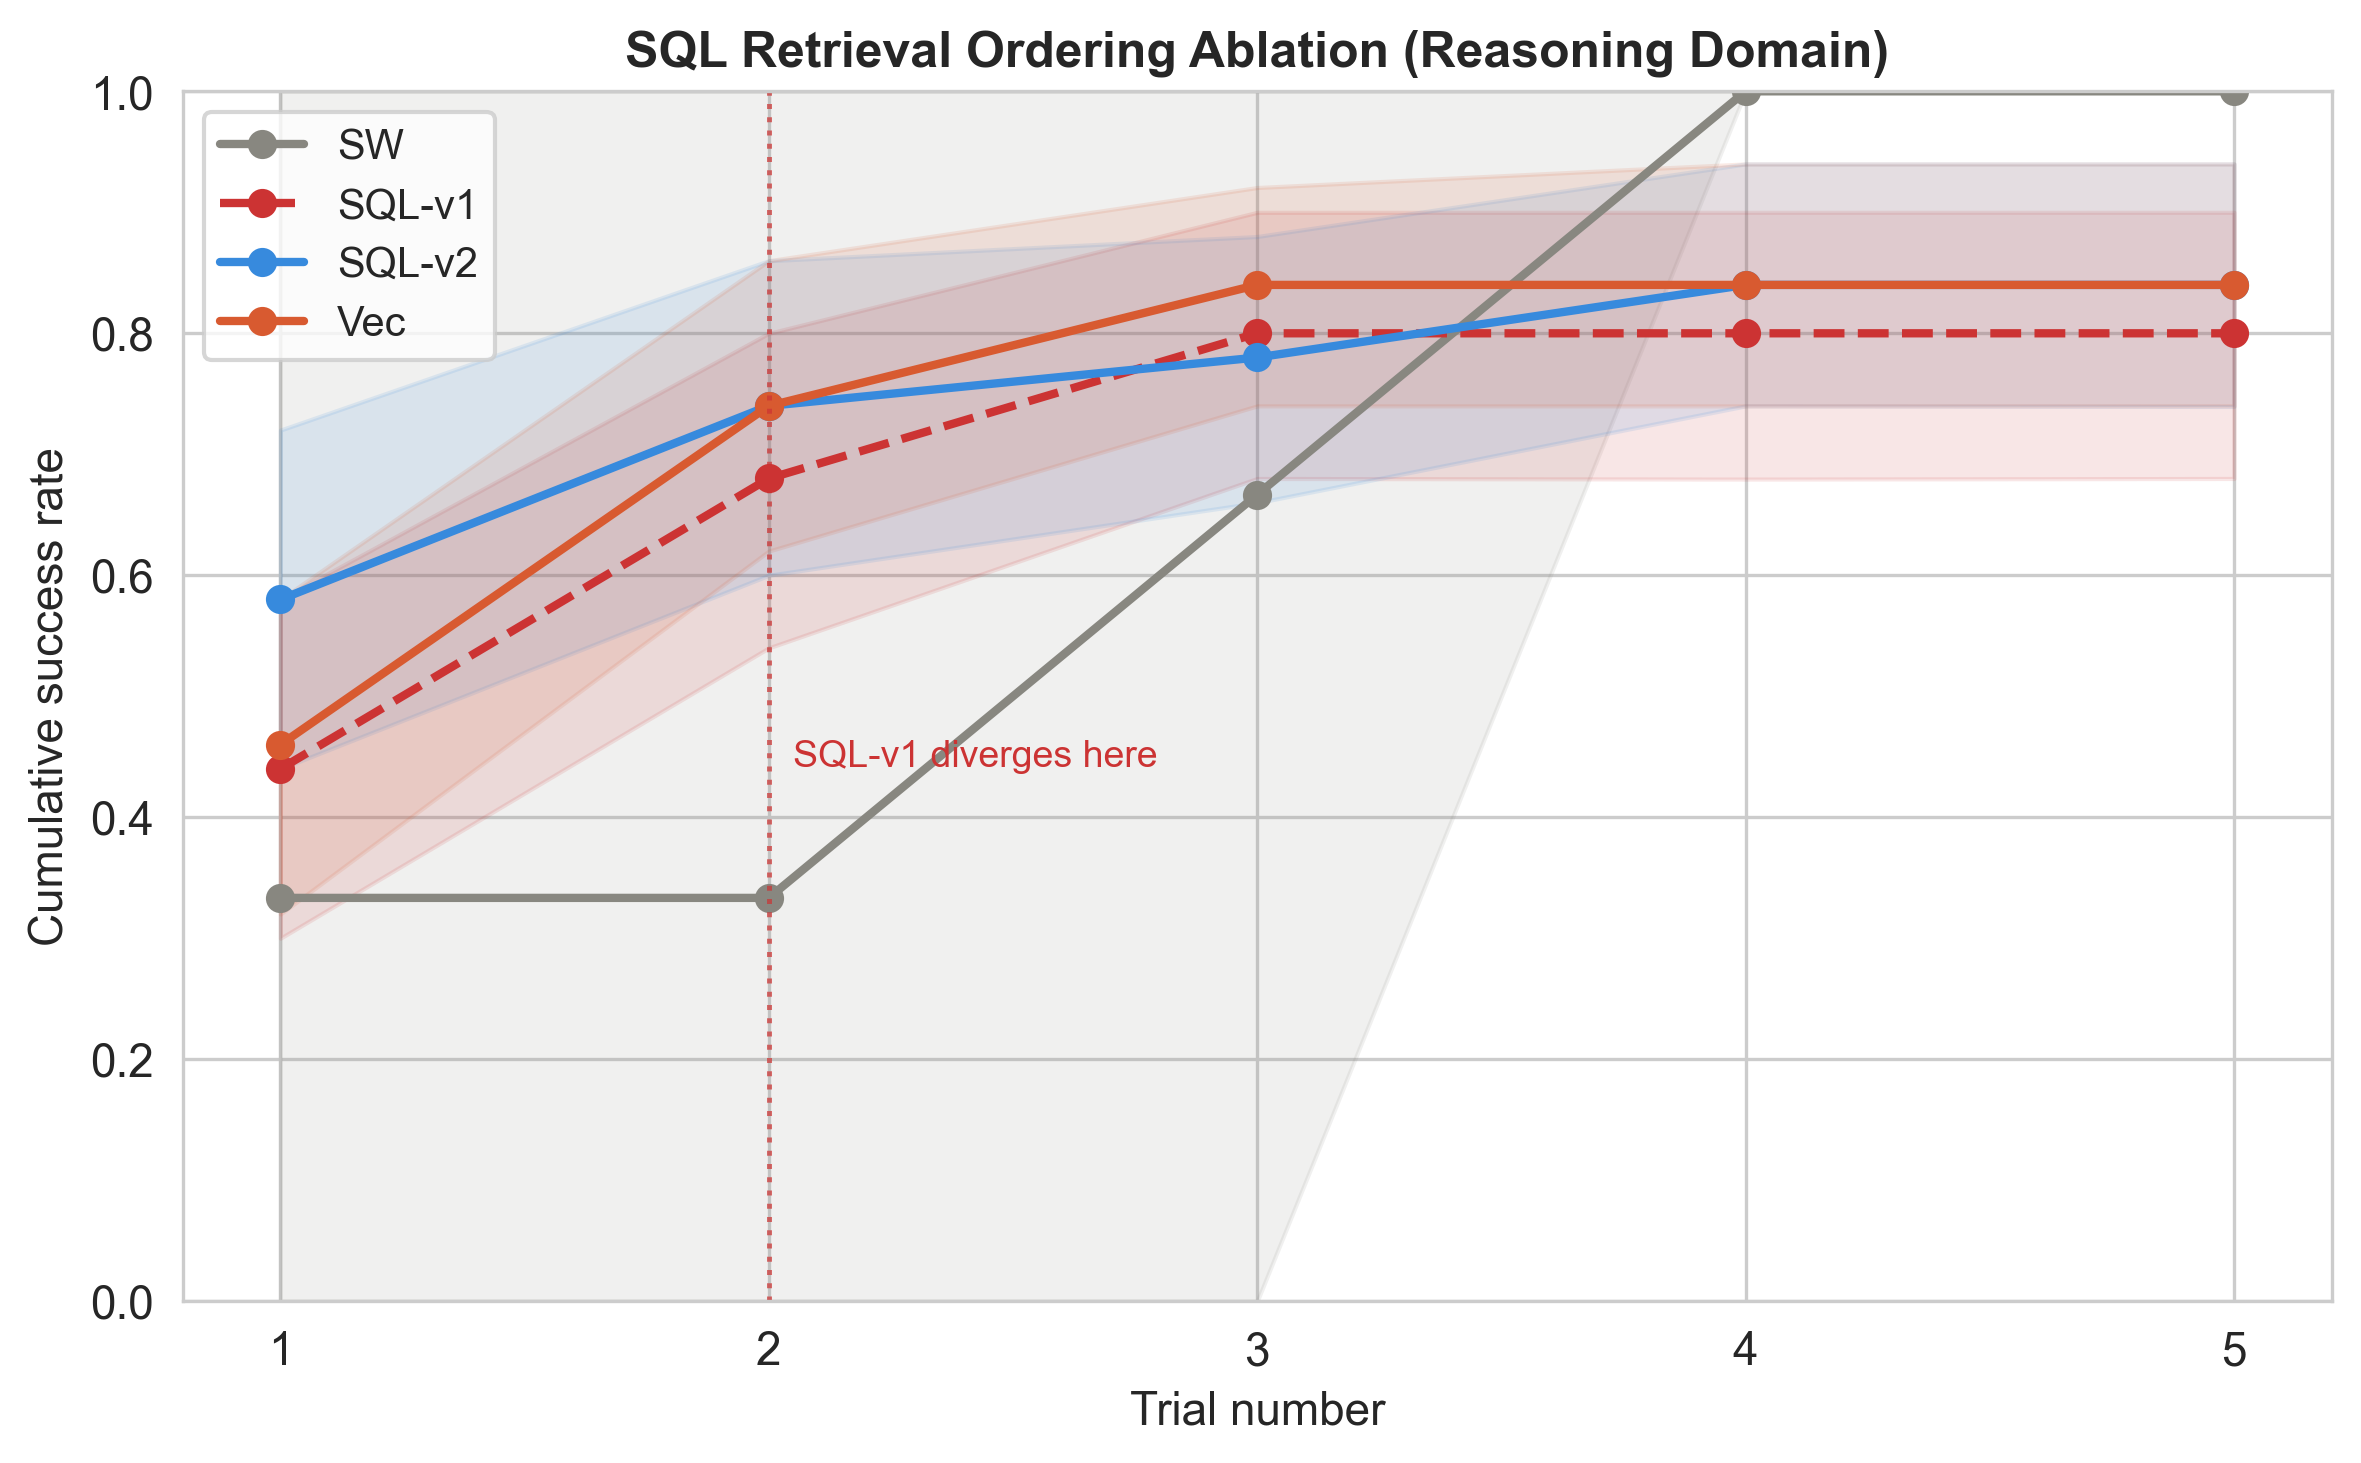
\includegraphics[width=0.85\linewidth]{sql_ordering_ablation.png}
\caption{
  Success curves for all four reasoning conditions across trials 1--5.
  SQL-v1 (success-first ordering) diverges from all other conditions at
  trial 2, where it begins retrieving past successes rather than failures.
  SQL-v2 (failure-first ordering) recovers to parity with Vector DB by
  trial 5. Error bars show 95\% bootstrap confidence intervals ($n{=}50$
  tasks, 1{,}000 resamples).
}
\label{fig:ordering}
\end{figure}

\subsection{Tool-Use Domain (BFCL multiple\_function)}

All three backends achieve 100\% success@5 on the BFCL
\texttt{multiple\_function} split ($n{=}20$). Despite the harder
disambiguation requirement, GPT-4o solves nearly all tasks on the first
attempt: SW and Vec achieve 100\% success@1, while SQL-v2 reaches 95\%
(19/20), with the one failure recovered by trial 2. The ceiling effect
observed on the simple split persists entirely on the
\texttt{multiple\_function} split, providing no signal for backend
differentiation. SW achieves the lowest mean token cost (966 tokens per
task, \$0.0048 per solved task), but this advantage is attributable to
task simplicity rather than retrieval efficiency. We discuss the benchmark
selection implications in Section~\ref{sec:discussion}.

\subsection{Sample Efficiency}

Vec requires only 48 episodes to reach 70\% cumulative success on
reasoning, compared to 88 for SQL-v2, 99 for SW, and 121 for SQL-v1. The
large gap between Vec and SW (48 vs.\ 99 episodes) indicates that semantic
retrieval produces meaningful signal earlier in the run, before the memory
database is large enough for recency-based heuristics to work well.
SQL-v1's 121-episode requirement reflects the warm-up confound: until
approximately 20 tasks have been run, even failure-first ordering has few
failure episodes to surface.

\subsection{Model Generalisability (GPT-4o-mini)}
\label{sec:miniresults}

To assess whether the retrieval ordering finding generalises beyond GPT-4o,
we ran all three reasoning-domain conditions (SW, SQL-v2, Vec) using
GPT-4o-mini on the same 50 HotpotQA tasks with the same fixed seed.
Table~\ref{tab:mini} shows the results alongside GPT-4o baselines (in
italics).

Two patterns emerge. First, first-attempt accuracy drops sharply across
all backends: Vector DB suffers the largest single-shot degradation
($-24$pp at success@1, from 70.0\% to 46.0\%), while SW declines least
($-8$pp, 58.0\% to 50.0\%). This suggests that GPT-4o-mini extracts less
value from semantically retrieved reflections on the first attempt,
consistent with a weaker base capacity for context utilisation. Second,
success@5 gaps narrow substantially: SW ($-2$pp), SQL-v2 ($-4$pp), Vec
($\pm 0$pp). Vector DB is fully robust at the five-attempt ceiling,
matching its GPT-4o performance exactly (84.0\%). These results indicate
that Reflexion iteration substantially compensates for the weaker base
model across all three backends.

The backend ranking at success@5 shifts modestly: with GPT-4o all three
converge to 84--86\%; with GPT-4o-mini, SW and Vec tie at 84.0\% while
SQL-v2 trails at 80.0\%. The SQL failure-first ordering advantage, while
preserved in direction, is smaller under GPT-4o-mini, suggesting the
structured retrieval benefit scales with the model's capacity to apply
failure-specific lessons.

\begin{table}[h]
\centering
\caption{
  GPT-4o-mini vs.\ GPT-4o on the reasoning domain (HotpotQA, $n{=}50$).
  GPT-4o-mini values shown first; GPT-4o baseline in \textit{italics}.
  Bold marks the best GPT-4o-mini value in each column.
}
\label{tab:mini}
\small
\begin{tabular}{lccccc}
\toprule
Backend & success@1 & success@3 & success@5
  & Mean tokens & Cost/solved (\$) \\
\midrule
SW
  & \textbf{0.500} \textit{(0.580)}
  & 0.780 \textit{(0.840)}
  & \textbf{0.840} \textit{(0.860)}
  & 4{,}180 \textit{(3{,}966)}
  & 0.0155 \textit{(0.0152)} \\
SQL-v2
  & 0.440 \textit{(0.580)}
  & \textbf{0.800} \textit{(0.780)}
  & 0.800 \textit{(0.840)}
  & 4{,}543 \textit{(4{,}075)}
  & 0.0164 \textit{(0.0151)} \\
Vec
  & 0.460 \textit{(0.700)}
  & \textbf{0.840} \textit{(0.820)}
  & \textbf{0.840} \textit{(0.840)}
  & \textbf{4{,}131} \textit{(3{,}621)}
  & \textbf{0.0153} \textit{(0.0125)} \\
\bottomrule
\end{tabular}
\end{table}

% ---------------------------------------------------------------------------
\section{Discussion}
\label{sec:discussion}

\subsection{Signal-to-Noise Framework}

We propose a \emph{signal-to-noise} framework for reasoning about memory
backend choice in Reflexion systems. Define \emph{signal density} as the
fraction of retrieved episodes that are genuinely relevant to the current
task and failure mode.

\textbf{Sliding Window} retrieval has high density for very small databases
(every stored episode is recent and therefore likely relevant) but density
degrades as the agent accumulates diverse experience. Recency and relevance
are correlated only when task types cluster temporally, which is a dataset
property rather than a retrieval property.

\textbf{SQL} maintains stable precision via structured filters (domain,
\texttt{error\_type}). Density does not degrade as the database grows
because the filter scope constrains the candidate set. However, SQL cannot
capture semantic similarity across tasks with different surface-form error
types, and as our ablation shows, the ordering of results within the
filtered set critically determines whether the agent receives useful
error-diagnosis information.

\textbf{Vector DB} density peaks at medium database size (approximately
100--500 episodes in our experiments). At small sizes, high density is
achieved trivially; at large sizes, noise from semantically adjacent but
irrelevant episodes accumulates. The minimum similarity threshold of 0.55
partially mitigates degradation at scale.

\subsection{Practical Recommendations}

Based on our results, practitioners building Reflexion-style agents should:

\begin{enumerate}
  \item \textbf{Use failure-first retrieval ordering in any structured
    memory system.} The SQL-v1 ablation shows that this single design
    decision accounts for a 12pp difference in success@5, larger than the
    difference between any two backend classes.
  \item \textbf{Prefer Vector DB for tasks with high semantic diversity}
    (varied question types, diverse error distributions), where cross-task
    lesson transfer is valuable.
  \item \textbf{Prefer SQL for tasks with nameable, categorical error
    types} (syntax errors, wrong tool selection) where structured credit
    assignment by error category outperforms semantic similarity.
  \item \textbf{Avoid sliding window as a default once the database exceeds
    approximately 50 episodes.} Its performance on success@1 is dominated
    by both SQL-v2 and Vec, and it offers no mechanism for targeted
    error-type-based lesson retrieval.
\end{enumerate}

\subsubsection*{Deployment Scenarios}

These guidelines map onto concrete real-world settings.

\subsubsection*{Customer Support Agents}

Customer support agents accumulate failure episodes as unresolved or
incorrectly resolved tickets. Failure-first SQL retrieval means the agent
surfaces lessons from structurally similar past failures rather than
rehearsing what previously worked, directly addressing the pattern of
repeating the same incorrect resolutions across semantically distinct
queries. The \texttt{error\_type} field in our schema maps naturally onto
support taxonomies such as billing errors, account access failures, and
policy misunderstandings, giving SQL's structured retrieval a well-defined
signal to filter on.

\subsubsection*{Code Generation Pipelines}

Code generation pipelines are the domain we could not evaluate directly
due to platform constraints, but the case is arguably stronger there than
in our reasoning experiments. Code failures are precisely the kind of
categorically nameable errors (syntax, runtime, type, wrong output) that
SQL retrieval is designed for. An agent that has previously seen a
\texttt{NullPointerException} in a similar context should retrieve that
specific lesson rather than a recent reflection about an unrelated
algorithmic task. The error-type retrieval path in our SQL implementation
(\texttt{retrieve\_by\_error\_type}) was built with this use case in mind.

\subsubsection*{RAG-Based Research and Document Assistants}

RAG-based research and document assistants benefit most from Vector DB,
and specifically from its sample efficiency advantage. Our results show
Vec reaching 70\% cumulative success after only 48 episodes versus 99 for
sliding window. In a fresh deployment with no prior episode history, this
means a Vector DB-backed assistant becomes reliably useful roughly twice
as fast as a recency-based one. For use cases where the agent encounters
diverse question types across many topics (research assistance, technical
documentation lookup, cross-domain QA), semantic similarity retrieval
surfaces relevant past lessons even when surface-form phrasing and error
categories differ across tasks.

The common thread across all three scenarios is that the value of a
memory backend is determined not just by storage capacity but by retrieval
precision under the specific failure distribution of the target task. Our
signal-to-noise framework provides a principled basis for matching backend
to deployment context before committing to infrastructure.

\subsection{Limitations}

\paragraph{Code domain excluded.}
HumanEval \citep{chen2021humaneval} could not be evaluated on Windows due
to the \texttt{signal.SIGALRM} dependency in the execution harness. This
is the domain where SQL's \texttt{retrieve\_by\_error\_type} (syntax
vs.\ runtime vs.\ wrong output) was predicted to provide the largest
advantage. A Linux or Docker environment is required to complete this
evaluation.

\paragraph{Tool-use benchmark difficulty.}
Both BFCL splits tested (simple and \texttt{multiple\_function}) exhibit a
100\% success@5 ceiling across all backends, providing no signal for
backend differentiation. The \texttt{multiple\_function} split is harder
at success@1 for SQL-v2 (95\% vs.\ 100\%) but the five-attempt ceiling is
identical. Harder benchmarks are required: ToolBench G2/G3 multi-tool
chains \citep{qin2023toolllm} or API-Bank \citep{li2023apibank} involve
sequential tool use and partial rewards that would create the graded signal
needed to distinguish memory backends.

\paragraph{Limited replications.}
Primary results (GPT-4o, all domains) reflect one random seed per
condition. The GPT-4o-mini reasoning results provide a full replication
across model capability levels: all three backends (SW, SQL-v2, Vec) were
run with the same 50-task seed, confirming the qualitative ordering of
backends is preserved. Bootstrap confidence intervals are reported on
within-condition task variance, but cross-seed variance for the primary
conditions is not quantified. Three seeds per condition would provide more
reliable estimates of backend-specific effect sizes and is a priority for
future work.

\paragraph{Reflection quality not scored.}
The reflector's output quality (specificity, actionability, and accuracy)
was not scored in these experiments, as the \texttt{--score-reflections}
flag was not used to avoid additional API cost. Reflection quality is the
central mechanistic variable: better memory retrieval should produce
higher-quality reflections, not just better task outcomes. Scoring a random
sample would provide stronger mechanistic evidence for the semantic
retrieval hypothesis.

% ---------------------------------------------------------------------------
\section{Conclusion}
\label{sec:conclusion}

We present the first systematic comparison of memory retrieval strategies
for Reflexion-style LLM agents, evaluating Sliding Window, SQL, and Vector
DB backends across two task domains. Our main findings are as follows.
First, a retrieval ordering decision (whether failures or successes are
surfaced first) accounts for a 12 percentage point difference in success@5,
larger than the difference between any two backend classes. Second, Vector
DB achieves the highest first-attempt success rate and lowest token cost on
reasoning tasks, consistent with the semantic retrieval hypothesis. Third,
the tool-use domain exhibits a ceiling effect on the BFCL benchmark,
motivating the use of harder benchmarks in future work.

The retrieval ordering finding has immediate practical value: any Reflexion
implementation using structured memory should order retrieved episodes by
failure first. This is a one-line change that recovers performance
equivalent to semantic retrieval at a fraction of the infrastructure cost.

Future work should evaluate on the HumanEval code domain (Linux/Docker),
use harder tool-use benchmarks, run the $k$-ablation to completion to
quantify the noise accumulation effect in Vector DB, and score reflection
quality directly to close the mechanistic loop between retrieval strategy
and lesson quality.

% ---------------------------------------------------------------------------
\section*{Acknowledgements}
Experiments were conducted using the OpenAI API. Embeddings were computed
with \texttt{sentence-transformers} \citep{reimers2019sentencebert}. Vector
storage was provided by ChromaDB. All data and code are publicly available
at \url{https://github.com/shilojeyaraj/reflexion-memory-study}.

% ---------------------------------------------------------------------------
\bibliographystyle{plainnat}
\bibliography{references}

\end{document}